\documentclass[a4paper,
fontsize=11pt,
%headings=small,
oneside,
numbers=noperiodatend,
parskip=half-,
bibliography=totoc,
final
]{scrartcl}

\usepackage{synttree}
\usepackage{graphicx}
\setkeys{Gin}{width=.6\textwidth} %default pics size

\graphicspath{{./plots/}}
\usepackage[ngerman]{babel}
%\usepackage{amsmath}
\usepackage[utf8x]{inputenc}
\usepackage [hyphens]{url}

\usepackage[colorlinks, linkcolor=black,citecolor=black, urlcolor=blue,
breaklinks= true]{hyperref}
\usepackage{booktabs} 
\usepackage[left=2.4cm,right=2.4cm,top=2.3cm,bottom=2cm,includeheadfoot]{geometry}
\usepackage{eurosym}
\usepackage{multirow}
\usepackage[ngerman]{varioref}
\setcapindent{1em}
\renewcommand{\labelitemi}{--}
\usepackage{paralist}
\usepackage{pdfpages}
\usepackage{lscape}
\usepackage{float}
\usepackage{acronym}
\usepackage{eurosym}
\usepackage[babel]{csquotes}
\usepackage{longtable,lscape}
\usepackage{mathpazo}
\usepackage[flushmargin,ragged]{footmisc} % left align footnote

\urlstyle{same}  % don't use monospace font for urls

\usepackage[fleqn]{amsmath}

%adjust fontsize for part

\usepackage{sectsty}
\partfont{\large}

%Das BibTeX-Zeichen mit \BibTeX setzen:
\def\symbol#1{\char #1\relax}
\def\bsl{{\tt\symbol{'134}}}
\def\BibTeX{{\rm B\kern-.05em{\sc i\kern-.025em b}\kern-.08em
    T\kern-.1667em\lower.7ex\hbox{E}\kern-.125emX}}

\usepackage{fancyhdr}
\fancyhf{}

\pagestyle{fancyplain}

\fancyhead[R]{\thepage}
%meta

\fancyhead[L]{R. Mumenthaler \\ %author
LIBREAS. Library Ideas, 24 (2014). % journal, issue, volume.
\href{http://nbn-resolving.de/urn:nbn:de:kobv:11-100215886}{urn:nbn:de:kobv:11-100215886}} % urn
\fancyhead[R]{\thepage} %page number
\fancyfoot[L] {\textit{Creative Commons BY 3.0}} %licence
\fancyfoot[R] {\textit{ISSN: 1860-7950}}

\title{\LARGE{Mit Expertenwissen zu Aussagen über künftige Entwicklungen –- der Horizon Report Higher Education}} %title %title
\author{Rudolf Mumenthaler} %author

\date{}

\begin{document}

\maketitle
\thispagestyle{fancyplain} 



\begin{center}
\sffamily{\textbf{ABSTRACT}}
\end{center}

\begin{abstract}
\small
Der Horizon Report Higher Education dient auch für Hochschulbibliotheken als wichtige Referenz zur Bewertung aktueller Trends und künftiger Entwicklungen. Der Autor stellt die dem Report zugrunde liegende Methode vor, beleuchtet diese kritisch und reflektiert die Aussagekraft der Prognosen. Die Stärken des Horizon Report liegen in der breiten Abstützung, der Offenheit des Verfahrens und der Publikation sowie der Ausarbeitung der von Expertinnen und Experten ausgewählten Themen. Gewisse Schwächen sieht der Autor in der Abhängigkeit von anderen Trendstudien sowie beim Auswahlverfahren der Trendthemen.
\end{abstract}

\begin{center}\rule{3in}{0.4pt}\end{center}


Als ich noch Verantwortlicher für Innovation an der ETH-Bibliothek
Zürich war, hatte ich den Termin im Februar für das Erscheinen des
Horizon Reports jeweils dick in der Agenda angestrichen. Die Aussagen zu
den Trends für die nächsten Jahre im Bereich Hochschulen schienen mir
auch für Hochschulbibliotheken sehr fundiert und zutreffend. Mit dem
Wechsel an die Fachhochschule HTW Chur 2012 veränderte sich auch mein
Interesse: nun war ich mehr am Entstehen als an den Ergebnissen eines
solchen Reports interessiert und ich beschloss, mich für das Advisory
Board zu melden. Ein entsprechender Aufruf findet sich auf der Homepage
des New Media Consortium, dem Herausgeber des Horizon Reports (
\url{http://www.nmc.org/}). Ich wurde in das Gremium aufgenommen und
habe in dieser Funktion an den beiden Horizon Reports Higher Education
2013 und 2014 mitgewirkt. Den dabei gewonnenen Blick hinter die Kulissen
des renommierten Trendberichts möchte ich im Folgenden für eine
kritische Würdigung des Reports und der ihm zugrunde liegenden Methode
nutzen.

\section*{Der Horizon Report Higher
Education}\label{der-horizon-report-higher-education}

Doch zunächst etwas Hintergrundinformation zum Horizon Report Higher
Education: Es handelt sich dabei um ein Projekt des New Media
Consortium, das sich mit aktuellen und künftigen Entwicklungen in der
Lehre befasst. Wobei es nicht nur den Bericht zu den Hochschulen gibt,
sondern mittlerweile auch Berichte für den Unterricht auf der Grundstufe
(K12), für Museen sowie für einzelne Länder und Regionen. Allen Reports
ist die Methode gemeinsam. Diese sieht vor, dass in einem angepassten
Delphi-Verfahren etwa 50 Expertinnen und Experten aus der ganzen Welt in
mehreren Schritten in die Eingrenzung der Thematik und Auswahl der
wichtigsten Trends mit einbezogen werden (vgl.
dazu~\url{http://horizon.wiki.nmc.org/Methodology}).

Zunächst stellen die federführenden Herausgeber und das Redaktionsteam
publizierte Studien und Berichte (Press Clippings) bereit, die durch die
Expertinnen und Experten ergänzt und kommentiert werden können.
Wichtigstes Arbeitsinstrument ist dabei das elaborierte Wiki, welches
alle Arbeitsschritte unterstützt
(\href{http://horizon.wiki.nmc.org}{http://horizon.wiki.nmc.org/}).
Neben den Reports und Publikationen stellt das Redaktionsteam auch eine
Liste von möglichen Schlüsseltechnologien im Wiki bereit. Diese kann und
soll durch die Expertinnen und Experten nicht nur kommentiert, sondern
auch durch eigene Themen ergänzt werden.

\begin{figure}[htbp]
\centering
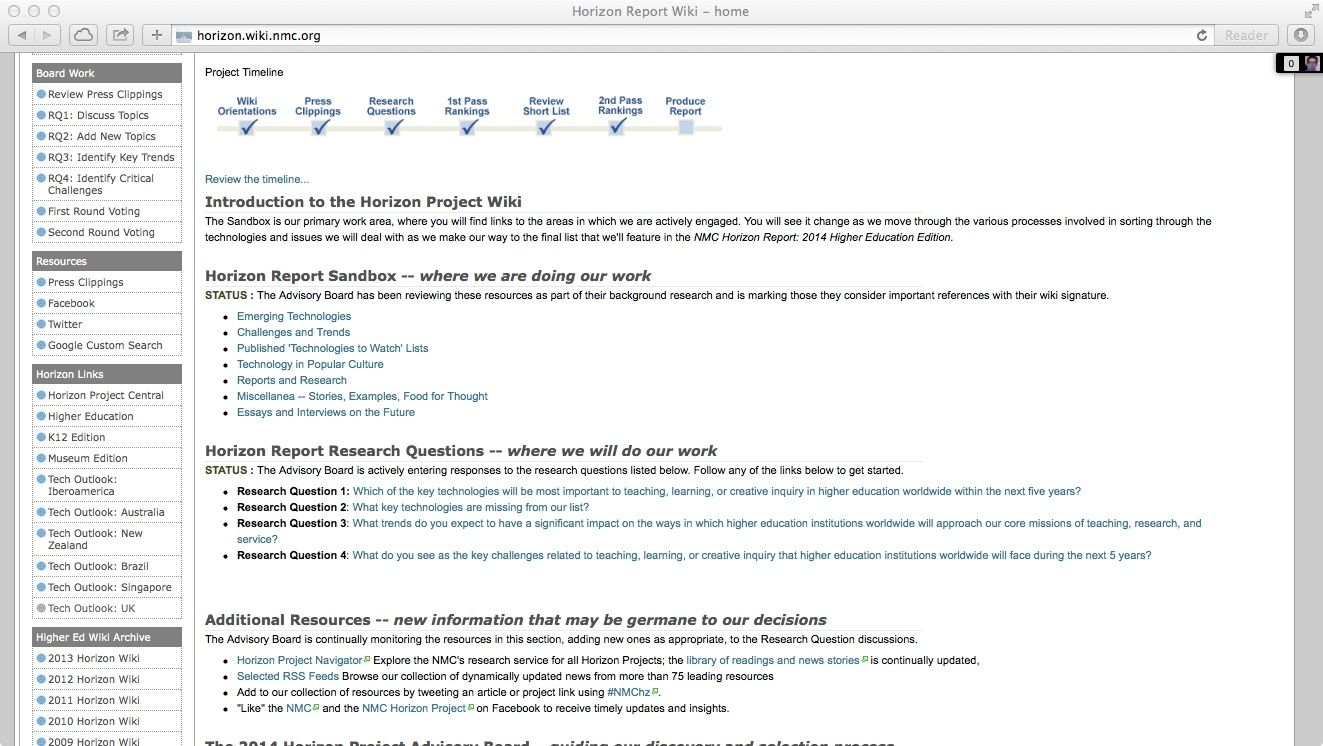
\includegraphics{./img/01-Horizon_Wiki.jpg}
\caption{Das Wiki des Horizon Report mit den Phasen und den
Forschungsfragen (Quelle: \url{http://horizon.wiki.nmc.org/home},
besucht 30.01.2014}
\end{figure}

Folgende vier Forschungsfragen werden in der ersten Phase im Wiki
diskutiert, kommentiert und gewichtet (hier in einer eigenen Übersetzung
der Fragen im Wiki \url{http://horizon.wiki.nmc.org/Methodology}):~

\begin{enumerate}
\def\labelenumi{\arabic{enumi}.}
\item
  Welche Schlüsseltechnologien werden weltweit in den nächsten fünf
  Jahren für Lehre, Lernen oder Studium an Hochschulen am wichtigsten
  sein?
\item
  Welche Schlüsseltechnologien vermissen Sie in der Liste {[}gemeint ist
  die im Wiki publizierte Liste der Technologien{]}?
\item
  Von welchen Trends erwarten Sie, dass sie einen bedeutenden Einfluss
  auf die Erfüllung der Kernaufgaben von Hochschulen weltweit in den
  Bereichen Lehre, Forschung und Dienstleistung haben werden?
\item
  Worin sehen Sie die Schlüsselherausforderungen in Bezug auf Lehre,
  Lernen und kreatives Studium, denen Hochschulen weltweit in den
  nächsten fünf Jahren gegenüberstehen?
\end{enumerate}

Gegenüber der ursprünglichen Version des Horizon Report, der sich noch
ausschliesslich auf die Technologien konzentrierte, wurden in den
letzten beiden Jahren die Aspekte \enquote{allgemeine Trends} und
\enquote{Herausforderungen} aufgenommen und somit der Fokus des Reports
erweitert. Die Technologien werden in mehrere Themenbereiche gegliedert:
Im aktuellen Jahrgang waren dies Consumer Technologies, Digital
Strategies, Internet Technologies, Learning Technologies, Social Media
Technologies, Visualization Technologies und Enabling Technologies. Die
komplette Liste findet sich im öffentlich zugänglichen Teil des
Wikis:~\url{http://horizon.wiki.nmc.org/Horizon+Topics} (besucht
19.12.2013). Die durch das Redaktionsteam erstellte Liste der
Schlüsseltechnologien war für den Report 2014 bereits sehr umfassend,
weshalb es nur noch wenige Ergänzungen durch die externen Expertinnen
und Experten gab.

Die Themen wurden also bereits gut vorbereitet. Im Prinzip stand es den
Expertinnen und Experten frei, die Liste komplett umzubauen, neue Themen
einzubringen und diese zu gewichten. Allerdings war die Zeit dafür sehr
knapp. Die Mitglieder des Advisory Board hatten nur zwei Wochen Zeit für
die Diskussion und Ergänzung der Themen (vom 8. bis 20. Oktober 2013),
wobei die Frist um eine Woche verlängert wurde. Für die Bewertung der
Themen stand eine Woche zur Verfügung. Anschliessend wertete das
Redaktionsteam die Bewertung durch das Advisory Board aus und erstellte
eine \enquote{Short List} mit den vier wichtigsten Themen pro
Zeithorizont (1 Jahr, 2-3 Jahre, 4-5 Jahre), und zwar jeweils für alle
drei Fragen nach Schlüsseltechnologien, Trends und Herausforderungen.
Aus den vom Redaktionsteam erstellten Listen konnten die Expertinnen und
Experten je ein Thema abwählen (negative Selektion). Dafür hatten sie
zehn Tage Zeit (vgl.~\url{http://horizon.wiki.nmc.org/Timeline}).

Auf der Grundlage dieses Verfahrens erstellte das Redaktionsteam
schliesslich die Auswahl von je zwei Themen pro Zeithorizont und
Themenfeld (Technologien, Trends, Herausforderungen). Für die
Publikation des Reports bearbeitete das Redaktionsteam diese Themen noch
weiter, wobei die Rückmeldungen des Advisory Boards im Wiki verarbeitet
wurden. Den Entwurf des finalen Reports erhielten die Experten noch zur
Begutachtung, bevor er anfangs Februar 2014 veröffentlicht wurde.

\section*{Das Auswahlverfahren}\label{das-auswahlverfahren}

Wie schon angesprochen, wird für den Horizon Report ein spezielles
Delphi-Verfahren angewandt. Hier möchte ich einen Aspekt dieses
Verfahrens etwas genauer betrachten, und zwar die Bewertung der Themen
für die drei verschiedenen Zeithorizonte.

Die Expertinnen und Experten erhalten die Möglichkeit, für jedes der
drei Themenfelder (Technologien, Trends, Herausforderungen) jeweils
insgesamt 30 Punkte zu vergeben, wobei für jeden Zeithorizont (1 Jahr,
2-3 Jahre, 4-5 Jahre) jeweils 10 Punkte verteilt werden können.~

Man beginnt als Expertin oder Experte also mit den Technologien,
Zeithorizont ein Jahr, und kann hier 10 Punkte auf unterschiedliche
Themen verteilen -- pro Thema einen bis drei Punkte. Im nächsten Schritt
können für den Zeithorizont 2-3 Jahre wiederum 10 Punkte vergeben
werden, dann für den Zeithorizont 4-5 Jahre, wobei die Themen, denen
bereits Punkte vergeben wurden, in den nächsten Horizonten nicht mehr
zur Wahl stehen. Dasselbe Vorgehen gilt dann für die anderen Fragen zu
Trends und Herausforderungen.

Mich als Experten beschlich hier ein Unbehagen: Ich musste mich
entscheiden, ob eine bestimmte Technologie im nächsten Jahr oder erst in
2-3 Jahren oder in 4-5 Jahren bedeutsam sein wird. Wenn ich aber einer
Technologie bei einem Zeithorizont Punkte gebe, fällt sie für die
anderen Zeithorizonte weg. Wenn sich also die Expertinnen und Experten
zwar einig sind, dass eine Technologie bedeutsam ist, aber bei der
Einschätzung bezüglich des Zeithorizonts unterschiedlicher Meinung sind,
kann diese Technologie im Gesamtranking von weniger wichtigen
Technologien, bei denen man sich aber bezüglich des Zeithorizonts einig
ist, überholt werden. Ein anderer negativer Effekt dieser Methodik:
Nachdem ich die wichtigsten Technologien in den ersten Zeithorizonten
bereits bewertet hatte, blieb im Zeithorizont 4-5 Jahre noch
\enquote{der Rest}, also eher unwichtige Technologien (oder Trends und
Herausforderungen), die ich möglicherweise auch nicht so richtig
einschätzen konnte.~

Ich habe noch nicht die Lösung für eine bessere Methodik parat. Aber ich
würde eine Methode begrüssen, bei der die Expertinnen und Experten
zunächst die grundsätzliche Bedeutung einer Technologie bewerten und
anschliessend angeben können, in welchem Zeithorizont sie diese
Technologie für relevant halten. Möglicherweise wäre es sinnvoll, wenn
man ein Thema grundsätzlich in jedem Zeithorizont bewerten könnte und
dann bei der Auswertung nur jener Zeithorizont berücksichtigt würde, in
dem die meisten Punkte vergeben wurden.

\section*{Ergebnisse der Horizon Reports
2004-2014}\label{ergebnisse-der-horizon-reports-2004-2014}

Betrachten wir nur die Rubrik \enquote{technologies to watch}, also die
technischen Entwicklungen, die in den nächsten Jahren einen prägenden
Einfluss auf die universitäre Lehre haben sollen. Der Horizon Report
unterscheidet zwischen drei Zeithorizonten: ein Jahr, zwei bis drei
Jahre, vier bis fünf Jahre. Rein theoretisch sollte ein Trend zunächst
in der Rubrik 4-5 Jahre auftauchen und sich dann in Richtung 1 Jahr
bewegen. Dies kommt allerdings nur sehr selten vor. Alle drei Phasen
durchlief bisher einzig das Thema \enquote{Learning Analytics}, das 2011
zum ersten Mal im Zeithorizont 4-5 Jahre auftauchte, dann in den
folgenden Jahren im Zeithorizont 2-3 Jahre und im aktuellen Horizon
Report für 2014 im Zeithorizont 1 Jahr erschien (die Horizon Reports
sind u.a. auf der Homepage des NMC
publiziert:~\url{http://www.nmc.org/publications}).~

\begin{figure}[htbp]
\centering
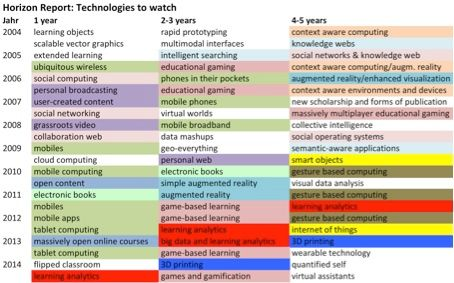
\includegraphics{./img/02-Themen_Horizon.jpg}
\caption{Wichtigste Technologien seit 2004, Themen farblich zu Clustern
zusammengefasst (eigene Darstellung)}
\end{figure}

Andere Themen dümpeln über mehrere Jahre in einem der Zeithorizonte, um
dann zu verschwinden, andere tauchen gleich im Zeithorizont 1 Jahr auf,
ohne vorher als wichtig erkannt worden zu sein. Beispiele für das
Dümpeln im Horizont 4-5 Jahre sind \enquote{context aware computing} und
\enquote{gesture based computing}. Letzteres Thema war 2010-2012 drei
Mal im Zeithorizont 4-5 Jahre und wurde dann nicht mehr erwähnt.
Spitzenreiter ist hier jedoch \enquote{game based learning}, das unter
verschiedenen Bezeichnungen seit 2005 in der Rubrik 2-3 Jahre verharrt.
Im neusten Report hat es diese Technologie unter der Bezeichnung
\enquote{games and gamification} wieder in dieselbe Rubrik geschafft.

Es gibt auch Themen, die nicht ganz linear den Weg von einem
Zeithorizont in den anderen geschafft haben: \enquote{augmented reality}
wird 2006 zum ersten Mal im Horizont 4-5 Jahre genannt, 2007 erneut
zusammen mit \enquote{context aware computing}, verschwindet dann aus
dem Ranking, um 2010 und 2011 im Zeithorizont 2-3 Jahre wieder genannt
zu werden. Weiter schafft es dieser Technologietrend (bisher) jedoch
nicht.

Und dann gibt es noch den Megatrend mobile Computing, der 2006 als
\enquote{phones in their pocket} erstmals im Horizont 2-3 Jahre erwähnt
wird, dort weitere zwei Mal auftritt und es dann in Varianten bis 2013
in den Zeithorizont 1 Jahr schafft (\enquote{mobiles}, \enquote{mobile
computing}, \enquote{mobile apps}, \enquote{tablet computing}), also 5
Jahre an der Spitze ausharrt.

Neben den Dauerbrennern gibt es jedoch auch Themen, die singulär
auftreten, wie zum Beispiel \enquote{cloud computing}, das 2009 im
einjährigen Horizont genannt wird, aber weder vorher noch nachher wieder
thematisiert wird.

Der oben kritisierte Aspekt, wonach im Zeithorizont 4-5 Jahre eher die
Themen zu finden sind, die nicht allgemein bekannt sind, hat auch eine
positive Seite: Hier findet man tatsächlich Themen, die noch nicht dem
grossen Hype entsprechen, und bei denen sich eine vertiefte
Beschäf\-tigung lohnt. Dafür bietet die ausführliche Behandlung der Themen
im publizierten Report eine gute Gelegenheit. Hier finden sich also
durchaus \enquote{Perlen} -- wie zum Beispiel das Thema
\enquote{Quantified Self} im aktuellen Report.

Als aktiver Teilnehmer am Ranking und somit als \enquote{Experte} stelle
ich einige unerklärliche Ergebnisse fest. Als Teilnehmer der Runde 2014
erscheint mir unverständlich, dass der technologische Schlüsseltrend
\enquote{wearable technology} gar nicht genannt wird, nachdem er 2013
(Horizont 4-5 Jahre) einmal erwähnt worden ist. Dabei müssten doch
eigentlich Google Glass oder Smart Watch ein Thema sein, zumal diese
tragbaren Devices die Dozierenden (zum Beispiel in der
Prüfungssituation) vor neue Herausforderungen stellen dürften.
Erstaunlich finde ich auch, dass es 3D-Printing erst in den Zeithorizont
2-3 Jahre geschafft hat, zumal mittlerweile Dutzende von Makerspaces
oder FabLabs diese Technologie bereits einsetzen und die 3D-Printer
schon den Heimbereich erreicht haben.

Die Aussagekraft des Horizon Report wurde schon mehrfach untersucht,
u.a. von Sergio Martin (Martin, Sergio: New technology trends in
education: Seven years of forecasts and convergence. In: \emph{Computers
\& Education}, Band 57, 2011, S. 1893--1906.), der sie auf Grundlage
bibliometrischer Vergleichsanalysen mehrheitlich positiv würdigt.

\section*{Vergleich mit anderen
Prognosemethoden}\label{vergleich-mit-anderen-prognosemethoden}

Welche Themen weltweit interessieren, zeigt Google Trends an
(\url{http://www.google.com/trends/} ). Hier wird natürlich kein Bezug
zur Hochschullehre geschaffen, jedoch zeigt ein Vergleich der aktuellen
Topthemen des Horizon Report 2014, dass andere -- nicht erwähnte
Technologien -- die Welt deutlich intensiver beschäftigen.

\begin{figure}[htbp]
\centering
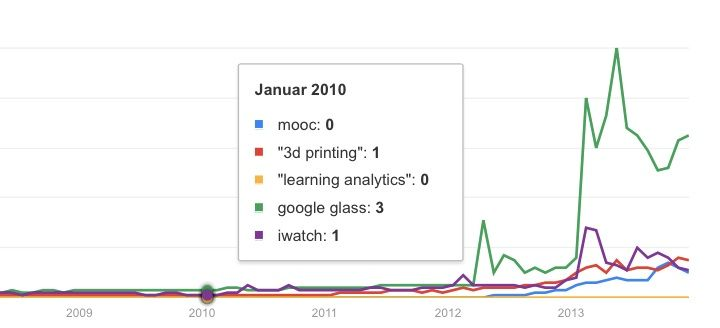
\includegraphics{./img/03-Google_Trends.jpg}
\caption{ausgewählte Themen bei Google Trends (die Legende zeigt aus
Gründen der Lesbarkeit die Werte für einen früheren Zeitpunkt,
massgeblich sind die Werte für 2013), zuletzt besucht: 19.12.2013}
\end{figure}

Hier liegen im Jahr 2013 Google Glass, 3D Printing, iWatch, und MOOCs
klar vor den beiden Favoriten des Horizon Report Learning Analytics und
Flipped Classroom.~

Ein Vergleich mit dem Gartner Hype Cycle for emerging technologies zeigt
einige Parallelen und einige deutliche Unterschiede (vgl. dazu die
Zusammenfassung und die Grafik zum Hype Cycle 2013
(\url{http://www.gartner.com/newsroom/id/2575515}). Gartner hat mit dem
Hype Cycle eine Methode und Präsentationsform für Technologietrends
entwickelt, die weltweit stark beachtet wird. Es werden hier neue
Technologien und deren Reifegrad ermittelt sowie der Zeitpunkt, bis zu
dem die Technologien produktiv werden dürften. Die Methode postuliert,
dass jede Technologie einem bestimmten Zyklus folgt: vom
Technologietreiber über den Hype, der leicht ironisch Gipfel der
überhöhten Erwartungen genannt wird, über das Tal der Tränen
(beziehungsweise der Desillusionierung) über die Kurve der Erleuchtung
hin zum Plateau der Produktivität. Im Unterschied zum Horizon Report ist
der Bericht von Gartner jedoch nicht offen zugänglich, mit Ausnahme der
Grafik und einer Zusammenfassung.

Die Themen \enquote{quantified self} und \enquote{virtual assistants},
die im Horizon Report 2014 im 4-5 Jahr-Horizont erwähnt werden, finden
sich im Gartner Hype Cycle von 2013 tatsächlich ebenfalls im Bereich 2-5
Jahre bis zur Erreichung des \enquote{Plateaus der Produktivität}.
\enquote{Gamification} sowie \enquote{Consumer 3D Printing} befinden
sich gerade auf dem \enquote{Gipfel der überhöhten Erwartungen} (beide
mit Zeithorizont 5-10 Jahre) und Content Analytics -- eine allgemeinere
Richtung als Learning Analytics, aber durchaus vergleichbar -- ist
ebenfalls auf dem Hype ziemlich weit oben (5-10 Jahre). 3D Printing
befindet sich zudem im Geschäftsbereich schon fast im produktiven
Bereich. ~

\begin{figure}[htbp]
\centering
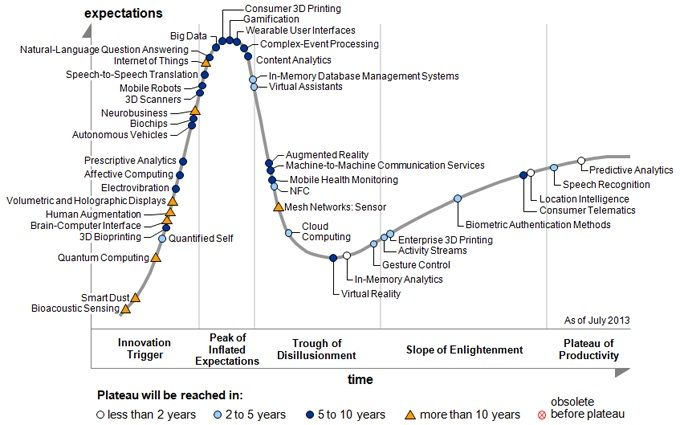
\includegraphics{./img/04-hype-cycle-2013.jpg}
\caption{Gartner Hype Cycle for Emerging Technologies, 2013
(\url{http://www.gartner.com/newsroom/id/2575515},besucht am
19.12.2013)}
\end{figure}

Im Gartner Hype Cycle für 2013 finden sich zudem auch einige Themen, die
in früheren Horizon Reports als wichtige Technologien genannt wurden --
in Klammern die erwarteten Jahre bis zur Produktivität: Gesture Control
(2-5), Virtual Reality (5-10, gerade im Tal der Desillusionierung),
Cloud Computing (2-5), Augmented Reality (5-10), Wearable User
Interfaces (5-10) sowie Internet of Things (über 10 Jahre). Eine
Beeinflussung der Ergebnisse des Horizon Report durch die jeweils im
Sommer veröffentlichte Gartner Studie ist nicht auszuschliessen -- auch
meine Einschätzung der künftigen Entwicklung wurde durch den Hype Cycle
sicherlich beeinflusst. So könnte also die Erwähnung des
\enquote{Quantified Self} im Gartner Hype Cycle 2013 dazu geführt haben,
dass er von den Experten und Expertinnen des Horizon Projekts
aufgenommen und für wichtig eingestuft wurde.

\section*{Fazit}\label{fazit}

Der Horizon Report Higher Education liefert eine vielbeachtete Vorschau
auf künftige Entwicklungen im Bereich der Hochschulbildung. Bei den
Ergebnissen fällt auf, dass sich einige Themen dauerhaft etablieren und
sich nicht entlang des Zeithorizonts entwickeln. Andere Themen erweisen
sich als kurzlebige Hypes und versinken in Vergessenheit. Die Abgrenzung
zwischen Technologien und Trends ist nicht immer scharf. Durch die
ausführliche Dokumentation der Themen bietet der Horizon Report eine
fundierte Übersicht über die aktuellsten Fragen (Technologien, Trends
und Herausforderungen) für Einrichtungen der Hochschulbildung. Es lohnt
sich, nicht nur den Bericht zu lesen, sondern auch das Wiki zu
konsultieren. Und der Horizon Report ist vorbildlich transparent und
offen: alle Inhalte sind unter einer Creative Commons Attribution Lizenz
(CC-BY) veröffentlicht.

Bei der Methodik gibt es einige Punkte, die ich als kritisch betrachte:
der Zeitdruck, unter dem die Bewertungen erfolgen müssen, erschwert eine
gründliche Auseinandersetzung mit den einzelnen Themen. Die Vorbereitung
durch das Redaktionsteam ist für die Expertinnen und Experten angenehm,
spurt aber die Resultate schon stark vor. Auch die zur Verfügung
gestellte Literatur ist sehr nützlich für das Advisory Board, doch wird
dieses dadurch möglicherweise beeinflusst. Die Möglichkeit, ein Thema
nur jeweils einem Zeithorizont zuzuordnen, verfälscht eventuell das
Ranking. Tendenziell dürften die wichtigen Themen schon in den
Zeithorizonten 1 Jahr und 2-3 Jahre genannt werden, wodurch für die
langfristige Rubrik die eher weniger bekannten Themen verbleiben. Wobei
dies den positiven Effekt hat, dass hier neue Themen entdeckt werden
können.

Letztlich geben bei einer Delphi-Methode eine bestimmte Anzahl
Expertinnen und Experten ihre persönliche Einschätzung der künftigen
Entwicklung ab. Die Intelligenz der Menge sorgt auf diesem Weg für
plausible Resultate, aber auch für wenige Überraschungen. Die Stärke des
Horizon Report besteht darin, dass allgemeine Trends und Entwicklungen
auf die Situation an Hochschulen heruntergebrochen werden. Zukunft lässt
sich mit der Methode nicht vorhersagen, aber die eigene Einschätzung
wird durch die Expertenmeinung bestärkt oder auch relativiert. Nicht
zuletzt als Argumentationshilfe innerhalb der eigenen Institution -- sei
es für die strategische Ausrichtung oder für die Entwicklung neuer
Dienstleistungen -- spielt der Horizon Report eine wichtige Rolle.

Die Aussagen aus dem Horizon Report lassen sich bis zu einem gewissen
Grad auf Hochschulbibliotheken übertragen. Aber gerade die neuen Aspekte
allgemeine Trends und Herausforderungen beziehen sich exklusiver auf die
Hochschullehre und haben wenig Bezug zu den Bibliotheken. Vor diesem
Hintergrund ist nun die Idee entstanden, eine Bibliotheksversion des
Horizon Report in Angriff zu nehmen. Der geplante Horizon Report Library
Edition soll sich auf wissenschaftliche Bibliotheken fokussieren und
noch 2014 in einer ersten Fassung erscheinen.

\begin{center}\rule{3in}{0.4pt}\end{center}

\textbf{Prof.~Dr.~Rudolf Mumenthaler} ist seit Mai 2012 an der
Fachhochschule HTW Chur am Schweizerischen Institut für
Informationswissenschaft als Dozent tätig. Zuvor war er von 1997-2012 an
der ETH-Bibliothek Zürich zunächst als Leiter der Spezialsammlungen, ab
2009 als Leiter des Bereichs Innovation und Marketing tätig gewesen.
2013 und 2014 hat er als Experte im Advisory Board des Horizon Report
mitgewirkt.

\end{document}